\documentclass[conference,a4paper]{IEEEtran}
\usepackage[utf8]{inputenc}
\usepackage[T1]{fontenc}
\usepackage{babel}
\babelprovide[import,main]{spanish}
\usepackage{graphicx}
\usepackage{amsmath,amssymb}
\usepackage{booktabs}
\usepackage{array}
\usepackage{tikz}
\usetikzlibrary{positioning,arrows.meta}
\usepackage{cite}
\usepackage{url}

% Como en la plantilla: "Abstract" y numeración de secciones en romanos
\addto\captionsspanish{\renewcommand{\abstractname}{Abstract}\renewcommand{\tablename}{TABLA}\renewcommand{\figurename}{Fig.}}
\renewcommand{\thetable}{\Roman{table}}

\begin{document}

\title{Reconstrucción 3D de espacios\\mediante COLMAP y Gaussian Splatting}

\author{\IEEEauthorblockN{Agustín Schwerdt\textsuperscript{\dag1}, Andrés Goinhex\textsuperscript{\dag2}}
\IEEEauthorblockA{\textsuperscript{\dag}\textit{Facultad de Ingeniería. Ingeniería Electrónica}\\
\textit{Universidad Nacional del Comahue}\\
\texttt{\textsuperscript{1}agustinschwerdt@gmail.com - ING-12470}\\
\texttt{\textsuperscript{2}andresleo001@gmail.com - ING-10776}}}

\maketitle

\begin{abstract}
En este trabajo se reconstruyeron en 3D cuatro escenas de la facultad (un objeto sobre una mesa, dos aulas y un pasillo) a partir de un único video filmado con un celular, sin LiDAR y sin calibrar la cámara. Primero se estimó la trayectoria de la cámara y una nube de puntos dispersa con Structure from Motion (COLMAP con extracción y correspondencia de características en GPU y el mapper global GLOMAP). Después se entrenó un modelo de 3D Gaussian Splatting que permite ver la escena desde puntos de vista nuevos. Las cuatro reconstrucciones registraron el 100\,\% de los frames, con un error de reproyección medio entre 0,36 y 0,62 píxeles, y los renders alcanzaron entre 27,4 y 32,9\,dB de PSNR sobre frames no usados en el entrenamiento.
\end{abstract}

\section{Introducción}

Un vehículo inteligente debe resolver dos problemas relacionados: la \textbf{localización}, es decir, determinar su \textit{pose} (posición y orientación) relativa a un mapa del ambiente, y la \textbf{construcción de mapas}, que asume conocida la pose del vehículo. Como para localizarse hace falta un mapa y para construir el mapa hace falta conocer la pose, ambos problemas se resuelven en conjunto mediante el \textbf{mapeo y localización simultánea} (SLAM, por sus siglas en inglés), visto en la Unidad V de la materia \cite{catedraU5}.

En este proyecto se aborda ese problema usando solamente una cámara monocular convencional, en un ambiente estático. A partir de un video se estima el \textit{movimiento de la cámara} (su trayectoria) y la \textit{estructura 3D} de la escena, que son los dos objetivos de la reconstrucción por visión de la Unidad V. Como se procesa todo el video junto, es una versión \textit{offline} del problema, equivalente al \textit{Full SLAM}: se estiman la trayectoria y el mapa completos. Sobre esa reconstrucción se construye un modelo 3D fotorrealista que puede recorrerse virtualmente y sirve como \textit{gemelo digital} del entorno, por ejemplo para generar imágenes sintéticas o para probar algoritmos de percepción en simulación.

El trabajo se dividió en tres etapas: (1) la filmación de cuatro escenas, (2) la estimación de las poses de la cámara mediante Structure from Motion (SfM) y (3) el entrenamiento de un modelo de 3D Gaussian Splatting (3DGS) y su evaluación con métricas de calidad de imagen.

\section{Marco teórico}

\subsection{Modelo de la cámara}

Se usa el \textbf{modelo pinhole} con distorsión de la lente \cite{catedraU2}. Un punto 3D $\mathbf{X}$ se proyecta en la imagen, en coordenadas homogéneas, como
\begin{equation}
\mathbf{x} = \mathbf{K}\,[\,\mathbf{R}\;|\;\mathbf{t}\,]\,\mathbf{X},
\end{equation}
donde la matriz de calibración $\mathbf{K}$ contiene los \textbf{parámetros intrínsecos} (distancias focales y punto principal, en píxeles) y $\mathbf{R}$, $\mathbf{t}$ son los \textbf{parámetros extrínsecos}, es decir, la pose de la cámara. En este trabajo no se calibró la cámara: el SfM estima los intrínsecos y la distorsión una vez para todo el video, y los extrínsecos para cada frame. Esos parámetros se usan después para proyectar el modelo 3D sobre cada imagen durante el entrenamiento.

\subsection{Extracción de características: puntos característicos, correspondencias y RANSAC}

Para relacionar dos imágenes de la misma escena se buscan \textbf{puntos característicos} o puntos de interés (\textit{keypoints}). Una buena característica debe ser \textit{repetible}, para poder encontrarla en otras imágenes; por eso los puntos aparecen en zonas con textura y casi nunca en superficies lisas.

Se usó \textbf{SIFT} (\textit{Scale Invariant Feature Transform}) \cite{catedraU3}. Detecta los puntos con diferencias de gaussianas (DoG) a distintas escalas, lo que lo hace invariante a la escala, y describe cada punto con un vector de 128 dimensiones (histogramas de orientación del gradiente) invariante a la rotación y a cambios de iluminación (Fig.~\ref{fig:sift}).

\begin{figure}[htbp]
\centering
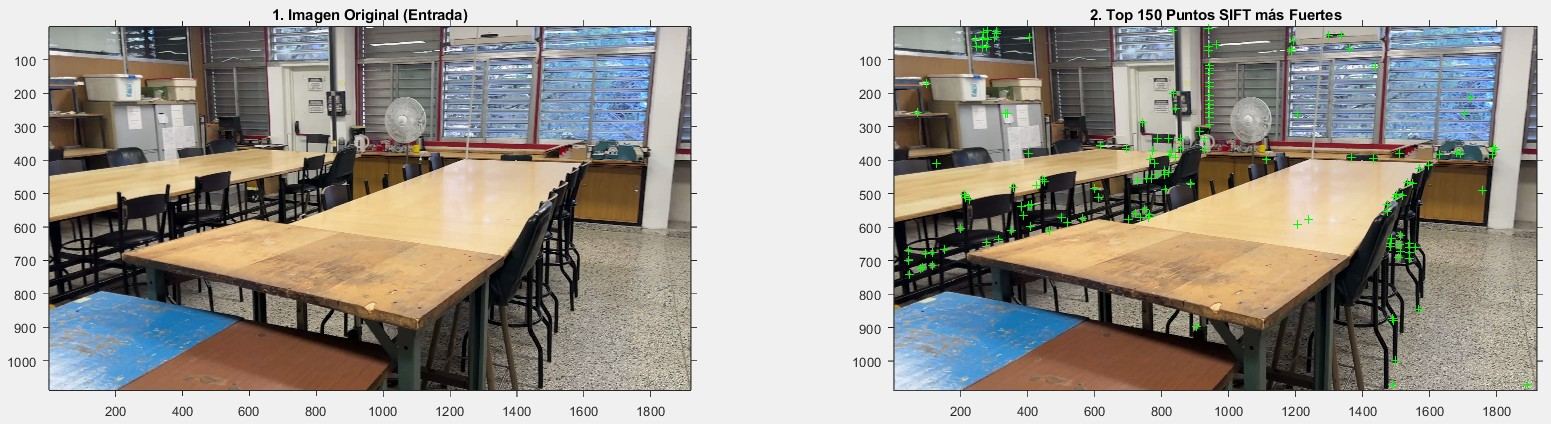
\includegraphics[width=\columnwidth]{fig/sift.jpg}
\caption{Frame del Aula B1 (izquierda) y los 150 puntos SIFT más fuertes detectados (derecha). Los puntos se concentran en bordes y zonas con textura (sillas, ventanas, estantes); casi no aparecen sobre las superficies lisas de las mesas.}
\label{fig:sift}
\end{figure}

La \textbf{correspondencia} (\textit{matching}) compara los descriptores de dos imágenes con una medida de distancia y empareja cada punto con su vecino más cercano. Muchas de esas correspondencias son incorrectas (\textbf{outliers}), por lo que se aplica \textbf{RANSAC} (\textit{RANdom SAmple Consensus}) \cite{catedraU3}: se elige al azar el mínimo subconjunto de correspondencias necesario para instanciar el modelo, que en este caso es la geometría entre las dos vistas (matriz fundamental o esencial, de la geometría epipolar). Después se cuentan las correspondencias que cumplen ese modelo dentro de una tolerancia de error, que forman el \textbf{conjunto de consenso}, y se repite. Se conserva el modelo con el mayor conjunto de consenso, cuyos elementos son los \textbf{inliers}. La Fig.~\ref{fig:ransac} muestra este proceso entre dos frames del aula: las correspondencias que se cruzan en el emparejamiento bruto son outliers, y desaparecen después de RANSAC.

\begin{figure}[htbp]
\centering
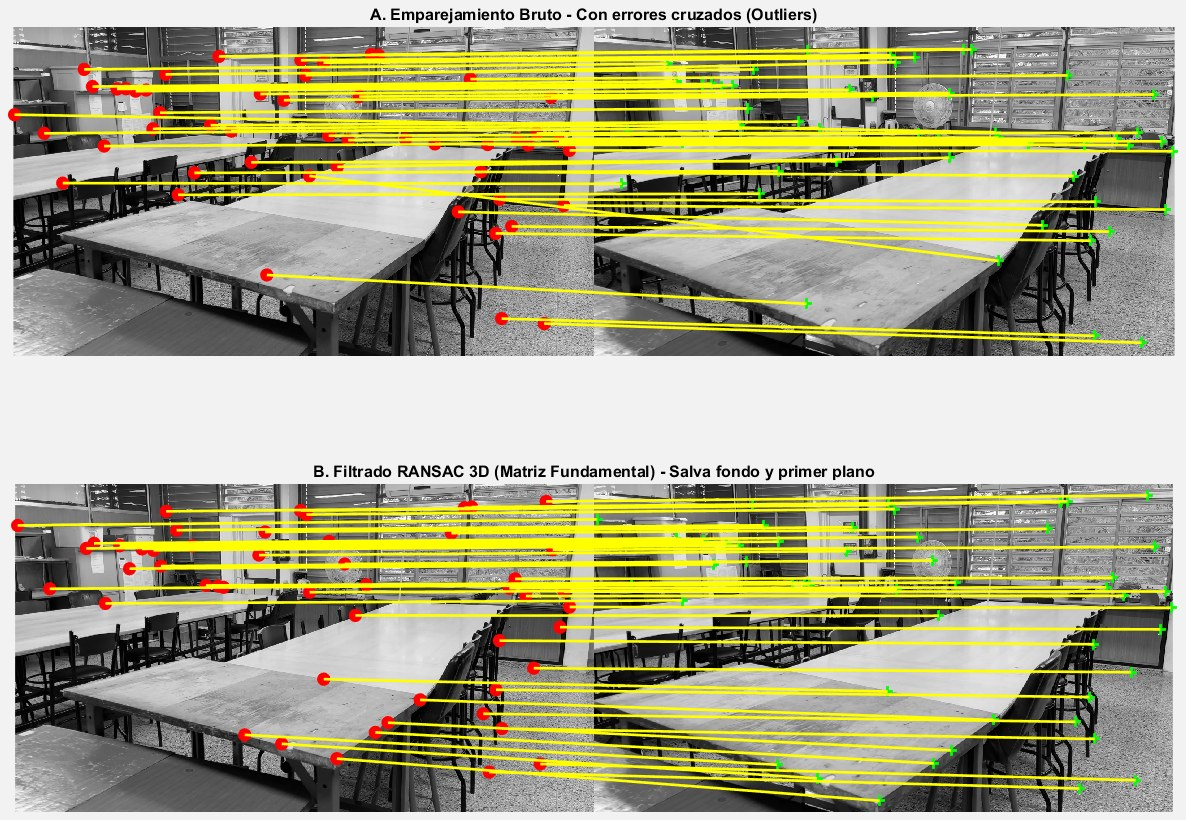
\includegraphics[width=0.9\columnwidth]{fig/ransac.jpg}
\caption{Arriba: correspondencias brutas de puntos SIFT entre dos frames, con outliers (líneas cruzadas). Abajo: inliers que quedan después de estimar la matriz fundamental con RANSAC.}
\label{fig:ransac}
\end{figure}

\subsection{Structure from Motion}

\textit{Structure from Motion} \cite{colmap} resuelve, a partir de múltiples vistas, los dos objetivos de la reconstrucción: el \textbf{movimiento de la cámara}, es decir, los parámetros extrínsecos (pose) de la cámara en cada imagen, y la \textbf{estructura 3D}, es decir, la posición 3D de los puntos característicos. También estima los parámetros intrínsecos y la distorsión, por lo que no hace falta calibrar la cámara.

En términos de SLAM, los puntos 3D cumplen el papel de \textit{landmarks} del mapa y las correspondencias filtradas con RANSAC resuelven la \textit{asociación de datos}.

El enfoque clásico, \textit{incremental}, agrega las cámaras de a una y reajusta todo el modelo cada vez. El enfoque \textit{global}, implementado en GLOMAP e incorporado a COLMAP \cite{colmap}, estima primero todas las rotaciones juntas, luego todas las posiciones de cámaras y puntos en un único problema, y suele ser más rápido. En ambos casos el resultado se refina con un \textit{bundle adjustment}: un ajuste por mínimos cuadrados de todas las poses y puntos que minimiza el \textbf{error de reproyección}, la distancia en píxeles entre donde se observa un punto en la imagen y donde lo proyecta el modelo de cámara de la ecuación (1).

Con una cámara monocular el SfM no puede conocer la escala real: una escena el doble de grande filmada desde el doble de distancia produce las mismas imágenes. Por eso el modelo tiene unidades arbitrarias.

\subsection{3D Gaussian Splatting}

El SfM entrega un mapa de puntos disperso: unas decenas o cientos de miles de puntos, que dejan huecos donde no hubo características (paredes lisas, pisos). Para obtener un modelo que se pueda \textit{ver} como una foto desde cualquier posición se usó 3D Gaussian Splatting (3DGS) \cite{kerbl2023}, una técnica de 2023 que no forma parte de los contenidos de la materia y es la parte novedosa de este proyecto.

\subsubsection{La idea}
En lugar de describir la escena con superficies (una malla de triángulos), 3DGS la describe con cientos de miles o millones de \textbf{gaussianas 3D}: pequeñas ``manchas'' difusas y semitransparentes con forma de elipsoide, como gotas de pintura en aerosol suspendidas en el espacio. Cada gaussiana tiene:
\begin{itemize}
\item una \textbf{posición} (su centro, la media $\boldsymbol{\mu}$);
\item una \textbf{forma y orientación}: tres escalas y una rotación, que definen un elipsoide (su matriz de covarianza $\boldsymbol{\Sigma}$). Puede ser redonda, alargada o aplanada como un disco;
\item una \textbf{opacidad} $\alpha$ entre 0 (transparente) y 1 (opaca);
\item un \textbf{color} que puede cambiar levemente según desde dónde se la mire, lo que permite representar brillos y reflejos.
\end{itemize}
Se usan gaussianas porque son suaves y derivables, y porque una gaussiana 3D proyectada sobre una imagen sigue siendo una gaussiana: una elipse 2D, fácil y rápida de dibujar.

\subsubsection{Cómo se genera una imagen}
Para obtener la imagen que vería una cámara con pose conocida, cada gaussiana se proyecta sobre el plano de imagen con el modelo de cámara de la ecuación (1). Esa proyección ``aplasta'' el elipsoide en una mancha 2D sobre la pantalla (de ahí el nombre \textit{splatting}). Luego las manchas se ordenan por distancia a la cámara y se superponen de adelante hacia atrás. El color de cada píxel es la mezcla de las gaussianas que lo cubren:
\begin{equation}
C = \sum_{i=1}^{N} c_i\,\alpha_i \prod_{j=1}^{i-1}(1-\alpha_j),
\end{equation}
donde $c_i$ y $\alpha_i$ son el color y la opacidad de la gaussiana $i$ en ese píxel. El producto representa la luz que todavía no fue tapada por las gaussianas que están delante: una gaussiana opaca cercana tapa a las que están detrás. Como este cálculo se reparte en la GPU por bloques de la imagen, el render es muy rápido, lo que permite recorrer la escena en tiempo real.

\subsubsection{Cómo se entrena}
Los parámetros de las gaussianas no se conocen de antemano: se aprenden a partir de las fotos, con el ciclo de la Fig.~\ref{fig:ciclo3dgs}:
\begin{enumerate}
\item \textbf{Inicialización}: se crea una gaussiana en cada punto de la nube dispersa del SfM, con el color de ese punto.
\item \textbf{Render}: se elige una foto de entrenamiento y se dibuja la escena desde la pose estimada para esa foto.
\item \textbf{Comparación}: se mide la diferencia entre el render y la foto real, combinando el error absoluto píxel a píxel con la similitud estructural (SSIM).
\item \textbf{Ajuste}: como todo el proceso es derivable, se calcula cómo cambia el error al modificar cada parámetro de cada gaussiana (\textit{gradiente}) y se los corrige un poco en la dirección que reduce el error (\textit{descenso del gradiente}).
\end{enumerate}
El ciclo se repite miles de veces (30\,000 en este trabajo) con fotos elegidas al azar. Es la misma idea de ajustar un modelo a los datos minimizando un error, como el ajuste por mínimos cuadrados, pero con millones de parámetros.

Al inicio no hay suficientes gaussianas para los detalles finos, por lo que durante la primera mitad del entrenamiento se aplica un \textbf{control adaptativo de densidad}:
\begin{itemize}
\item \textbf{Clonación}: donde falta detalle, se duplican gaussianas pequeñas.
\item \textbf{División}: las gaussianas demasiado grandes para representar un detalle se dividen en otras más chicas.
\item \textbf{Podado}: se eliminan las gaussianas casi transparentes, que no aportan a la imagen.
\end{itemize}
Por eso la cantidad de gaussianas crece durante el entrenamiento y después se estabiliza.

\begin{figure}[htbp]
\centering
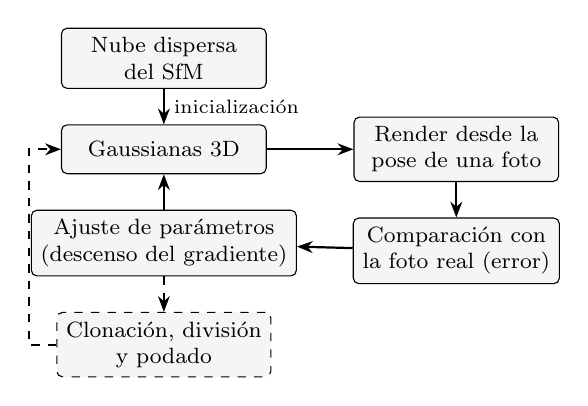
\begin{tikzpicture}[
  caja/.style={draw, rounded corners=2pt, minimum width=2.6cm, minimum height=0.62cm, align=center, font=\footnotesize, fill=gray!8},
  flecha/.style={-{Stealth[length=2mm]}, thick}, node distance=0.45cm and 0.5cm]
\node[caja] (sfm) {Nube dispersa\\del SfM};
\node[caja, below=of sfm] (g) {Gaussianas 3D};
\node[caja, right=1.1cm of g] (r) {Render desde la\\pose de una foto};
\node[caja, below=of r] (c) {Comparación con\\la foto real (error)};
\node[caja, below=of g] (a) {Ajuste de parámetros\\(descenso del gradiente)};
\node[caja, dashed, below=of a] (d) {Clonación, división\\y podado};
\draw[flecha] (sfm) -- node[right, font=\scriptsize]{inicialización} (g);
\draw[flecha] (g) -- (r);
\draw[flecha] (r) -- (c);
\draw[flecha] (c) -- (a);
\draw[flecha] (a) -- (g);
\draw[flecha, dashed] (a) -- (d);
\draw[flecha, dashed] (d.west) -- ++(-0.35,0) |- (g.west);
\end{tikzpicture}
\caption{Ciclo de entrenamiento de 3D Gaussian Splatting. El ciclo se repite 30\,000 veces; la densificación (línea discontinua) se aplica periódicamente durante la primera mitad.}
\label{fig:ciclo3dgs}
\end{figure}

\subsubsection{Diferencia con otros métodos}
La fotogrametría clásica construye una malla de triángulos, que tiene problemas con objetos finos, reflejos y vidrios, porque supone que cada punto se ve igual desde cualquier ángulo. Los NeRF (\textit{Neural Radiance Fields}) logran imágenes muy realistas usando una red neuronal, pero renderizar cada imagen es lento. 3DGS consigue una calidad similar a los NeRF con una representación explícita (una lista de gaussianas que se puede guardar en un archivo \texttt{.ply} y abrir en un visor), y el render es mucho más rápido.

Puede pensarse como un ``mapa'' del ambiente que, en vez de celdas fijas como una grilla de ocupación, usa elementos que se mueven, cambian de tamaño y guardan color y opacidad, construido integrando muchas imágenes tomadas desde poses conocidas.

\subsection{Métricas de calidad}

Para evaluar el modelo, siguiendo la evaluación que trae Nerfstudio \cite{nerfstudio}, se renderizan las poses de frames que no se usaron para entrenar y se comparan con las fotos reales mediante tres métricas:
\begin{itemize}
\item \textbf{PSNR} (dB): relación señal a ruido pico, basada en el error cuadrático medio (MSE) entre las imágenes. Más alto es mejor.
\begin{equation}
\mathrm{PSNR} = 10\log_{10}\!\left(\frac{\mathrm{MAX}^2}{\mathrm{MSE}}\right)
\end{equation}
\item \textbf{SSIM} (0 a 1): similitud estructural, que compara luminancia, contraste y estructura local. Más alto es mejor.
\item \textbf{LPIPS}: distancia perceptual calculada con una red neuronal, que se asemeja a cuánto se nota la diferencia a simple vista. Más bajo es mejor.
\end{itemize}

\section{Metodología}

\subsection{Captura de las escenas}

Se filmaron cuatro escenas con la cámara de un iPhone, a 1080p, moviéndose despacio y recorriendo la escena desde distintos ángulos (Tabla~\ref{tab:escenas}). La escena \textit{Lata} es un objeto pequeño (una lata de yerba) filmado en un recorrido circular a su alrededor. Las escenas \textit{Aula B1} y \textit{Aula B2} son dos laboratorios de la facultad, y \textit{Pasillo} es un recorrido en línea recta por un pasillo.

\begin{table}[htbp]
\caption{Escenas filmadas}
\label{tab:escenas}
\centering
\begin{tabular}{@{}llcc@{}}
\toprule
Escena & Recorrido & Orientación & Frames usados \\
\midrule
Lata     & circular alrededor del objeto & vertical   & 321 \\
Aula B1  & perímetro del aula            & horizontal & 432 \\
Aula B2  & dos vueltas por el aula       & vertical   & 899 \\
Pasillo  & lineal                        & horizontal & 617 \\
\bottomrule
\end{tabular}
\end{table}

\subsection{Pipeline de procesamiento}

El procesamiento se implementó en un cuaderno de Google Colab con una GPU NVIDIA L4 (24\,GB). La Fig.~\ref{fig:pipeline} resume las etapas:

\begin{enumerate}
\item \textbf{Extracción de frames}: con ffmpeg se toma un frame cada $k$ cuadros del video, para quedarse con la cantidad deseada, y se reduce la imagen a 1600\,px de lado mayor. Se mide además la nitidez de cada frame (varianza del laplaciano) para detectar frames movidos.
\item \textbf{SfM}: con \texttt{pycolmap} 4.2.1 compilado con CUDA se extraen las características SIFT y se calculan las correspondencias (\textit{matching}) secuenciales en la GPU (cada frame se compara con los 15 siguientes, ya que provienen de un video). Con esas correspondencias, GLOMAP estima las poses de cámara y la nube dispersa. Se usó un único modelo de cámara OpenCV (pinhole con distorsión) para todo el video.
\item \textbf{Conversión}: las poses se pasan al formato de Nerfstudio (\texttt{transforms.json}), cambiando de la convención de ejes de OpenCV a la de OpenGL.
\item \textbf{Entrenamiento}: se usa \textit{Splatfacto}, la implementación de 3DGS de Nerfstudio \cite{nerfstudio}, con el rasterizador gsplat, durante 30\,000 iteraciones. La densificación se aplica hasta la iteración 15\,000 y se podan las gaussianas con opacidad menor a 0,1. Al exportar se descartan además las gaussianas de opacidad muy baja. El 90\,\% de los frames se usa para entrenar y el 10\,\% restante para evaluar.
\item \textbf{Evaluación y exportación}: se calculan PSNR, SSIM y LPIPS sobre los frames de evaluación, se renderiza un video de recorrido y se exporta el modelo como archivo \texttt{.ply}, que puede abrirse en visores web de \textit{splats}.
\end{enumerate}

\begin{figure}[htbp]
\centering
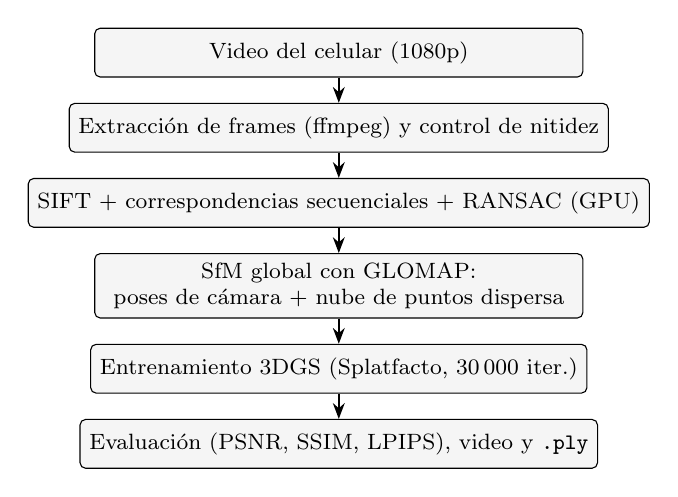
\begin{tikzpicture}[
  caja/.style={draw, rounded corners=2pt, minimum width=6.2cm, minimum height=0.62cm, align=center, font=\footnotesize, fill=gray!8},
  flecha/.style={-{Stealth[length=2mm]}, thick},
  node distance=0.32cm]
\node[caja] (v) {Video del celular (1080p)};
\node[caja, below=of v] (f) {Extracción de frames (ffmpeg) y control de nitidez};
\node[caja, below=of f] (s) {SIFT + correspondencias secuenciales + RANSAC (GPU)};
\node[caja, below=of s] (g) {SfM global con GLOMAP:\\ poses de cámara + nube de puntos dispersa};
\node[caja, below=of g] (t) {Entrenamiento 3DGS (Splatfacto, 30\,000 iter.)};
\node[caja, below=of t] (e) {Evaluación (PSNR, SSIM, LPIPS), video y \texttt{.ply}};
\draw[flecha] (v) -- (f); \draw[flecha] (f) -- (s); \draw[flecha] (s) -- (g);
\draw[flecha] (g) -- (t); \draw[flecha] (t) -- (e);
\end{tikzpicture}
\caption{Etapas del procesamiento.}
\label{fig:pipeline}
\end{figure}

\section{Resultados}

\subsection{Structure from Motion}

La Tabla~\ref{tab:sfm} resume los resultados del SfM. En las cuatro escenas se estimó la pose del 100\,\% de los frames y el error de reproyección medio quedó por debajo de 1 píxel, lo que indica que las poses y los puntos 3D son consistentes con las imágenes. Cada punto 3D se observa, en promedio, en entre 9 y 15 imágenes. El porcentaje de frames borrosos fue bajo en todos los casos (como máximo 4,6\,\% en Aula B2).

\begin{table}[htbp]
\caption{Resultados del Structure from Motion}
\label{tab:sfm}
\centering
\setlength{\tabcolsep}{4pt}
\begin{tabular}{@{}lcccc@{}}
\toprule
 & Lata & Aula B1 & Aula B2 & Pasillo \\
\midrule
Frames con pose           & 321/321 & 432/432 & 899/899 & 617/617 \\
Puntos 3D                 & 39\,817 & 112\,556 & 700\,338 & 162\,343 \\
Error de reproy. (px)     & 0,52 & 0,62 & 0,36 & 0,40 \\
Imágenes por punto        & 10,2 & 11,4 & 9,0 & 15,2 \\
Frames borrosos (\%)      & 3,1 & 0,0 & 4,6 & 0,2 \\
Tiempo de SfM (min)       & 3,5 & 15,6 & 106,9 & 31,7 \\
\bottomrule
\end{tabular}
\end{table}

La Fig.~\ref{fig:tray} muestra la trayectoria estimada de la cámara sobre la nube dispersa, vista desde arriba. Las trayectorias reproducen los recorridos realizados: un círculo alrededor de la lata, el perímetro del Aula B1, las dos vueltas en el Aula B2 y una línea recta en el pasillo. En términos de la materia, esta trayectoria es la \textit{localización} de la cámara (su pose en cada instante), y la nube dispersa es un \textit{mapa basado en features o landmarks} del entorno.
La Fig.~\ref{fig:camaras} muestra las mismas poses en 3D, dibujadas como pirámides dentro del modelo del Aula B1: cada pirámide indica dónde estaba la cámara y hacia dónde apuntaba en un frame.

\begin{figure}[htbp]
\centering
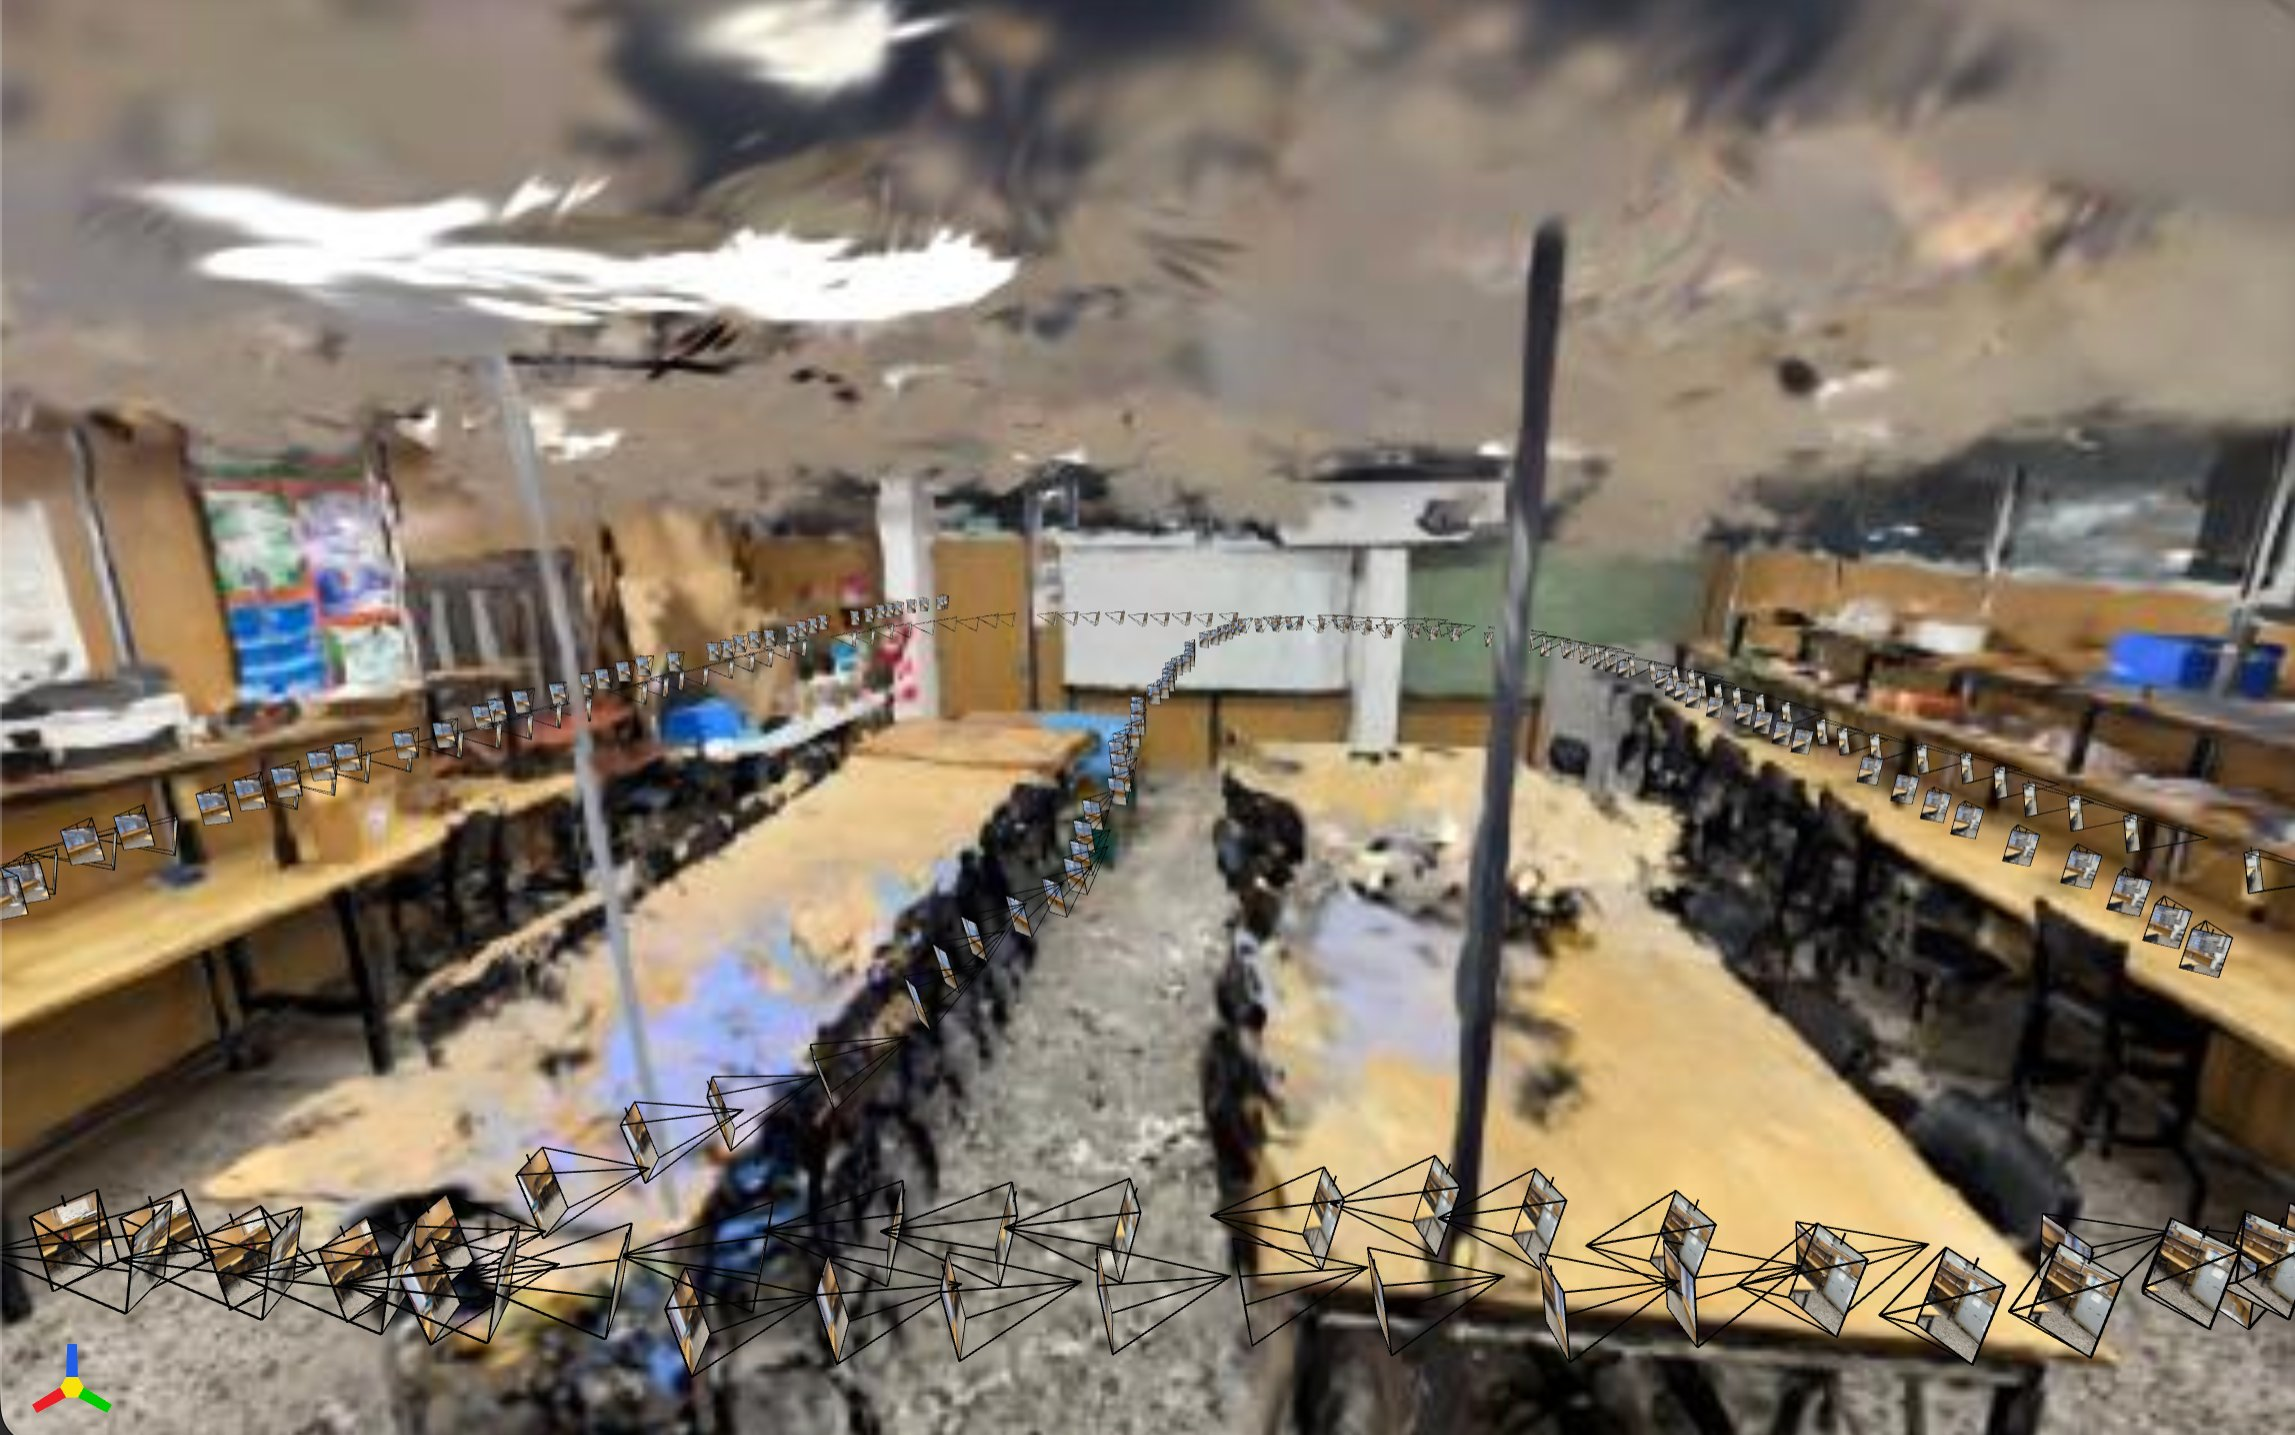
\includegraphics[width=0.82\columnwidth]{fig/camaras_sfm.jpg}
\caption{Poses de cámara estimadas por el SfM en el Aula B1, vistas en el visor de Nerfstudio durante el entrenamiento. Cada pirámide es un frame del video.}
\label{fig:camaras}
\end{figure}

\begin{figure}[htbp]
\centering
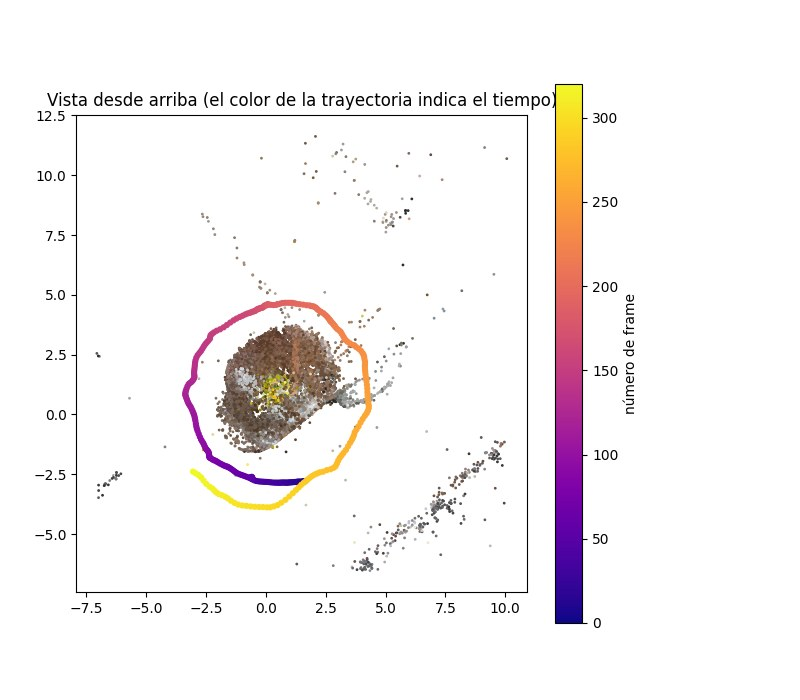
\includegraphics[width=0.49\columnwidth]{fig/tray_playadito.jpg}\hfill
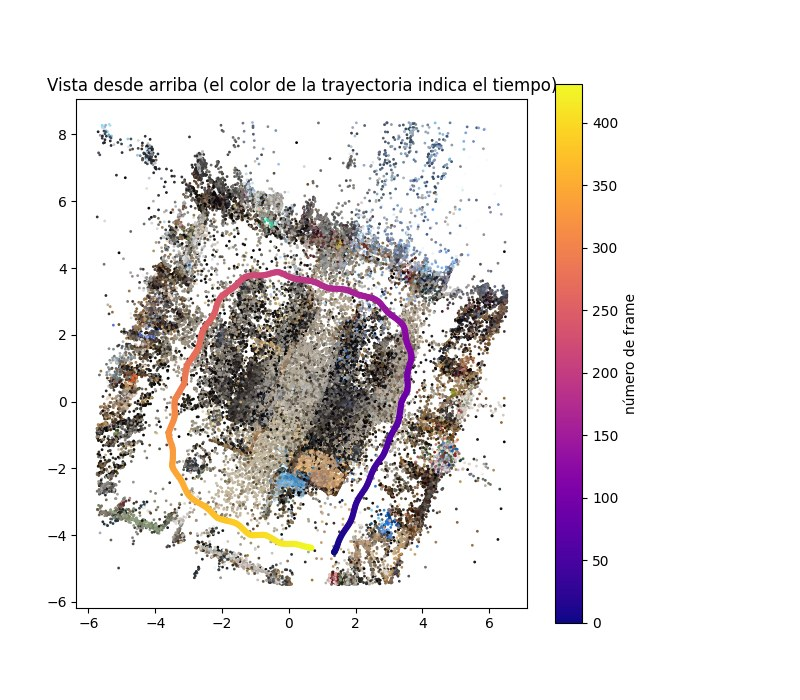
\includegraphics[width=0.49\columnwidth]{fig/tray_aulab1.jpg}\\[2pt]
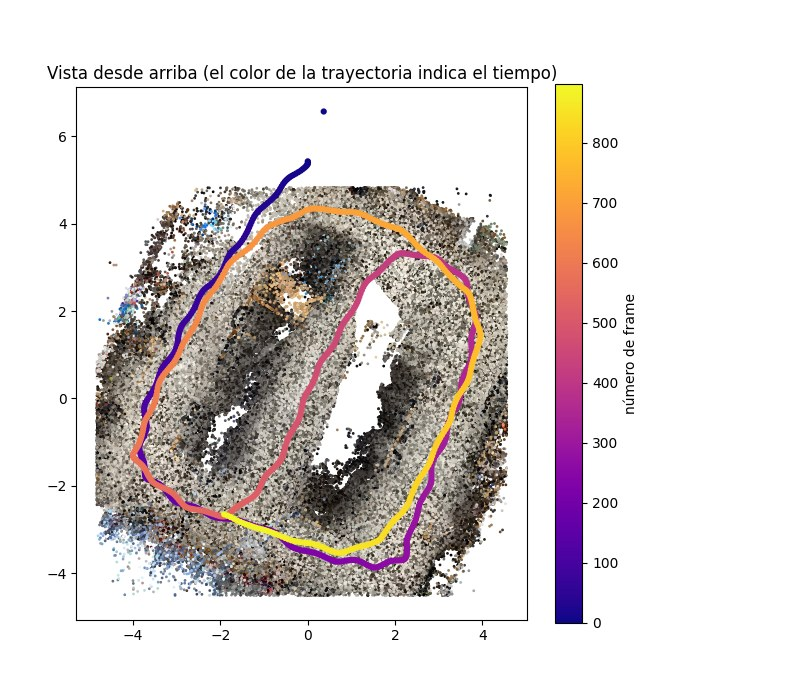
\includegraphics[width=0.49\columnwidth]{fig/tray_aulab2.jpg}\hfill
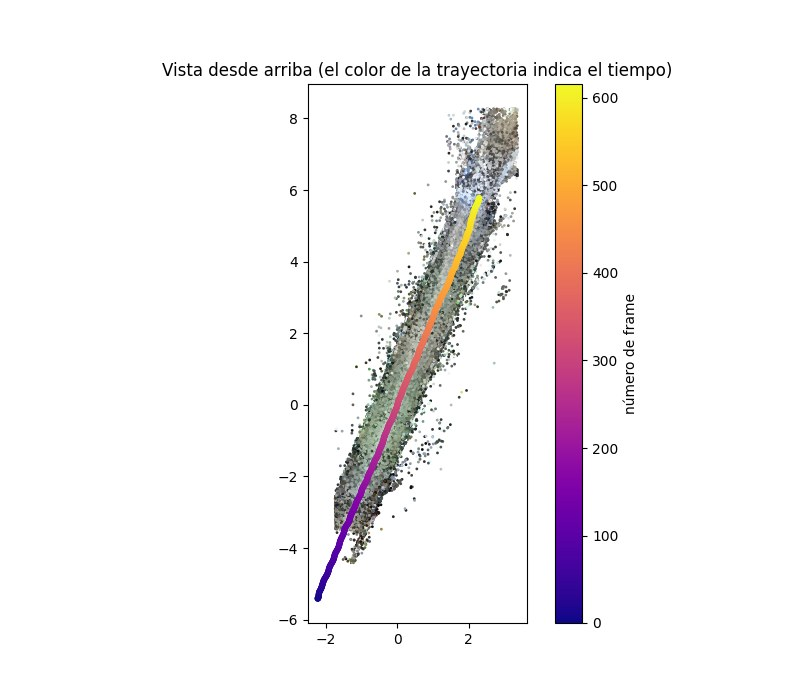
\includegraphics[width=0.49\columnwidth]{fig/tray_pasillo.jpg}
\caption{Nube dispersa y trayectoria de la cámara vistas desde arriba (el color indica el número de frame). Arriba: Lata y Aula B1. Abajo: Aula B2 y Pasillo. Unidades arbitrarias de COLMAP.}
\label{fig:tray}
\end{figure}

El tiempo de SfM creció mucho con el tamaño de la escena. En la escena Lata, la extracción SIFT tardó 7,7\,s, las correspondencias 33,6\,s y GLOMAP 166\,s. En Aula B2 esos tiempos fueron 32\,s, 548\,s y 5\,834\,s, respectivamente: la extracción y las correspondencias en GPU fueron rápidas, y la mayor parte del tiempo se la llevó la etapa de reconstrucción global, que corre en CPU.

\subsection{Gaussian Splatting}

La Tabla~\ref{tab:3dgs} presenta las métricas de calidad obtenidas sobre los frames de evaluación, junto con el tamaño de cada modelo.

\begin{table}[htbp]
\caption{Resultados de 3D Gaussian Splatting}
\label{tab:3dgs}
\centering
\setlength{\tabcolsep}{4pt}
\begin{tabular}{@{}lcccc@{}}
\toprule
 & Lata & Aula B1 & Aula B2 & Pasillo \\
\midrule
PSNR (dB) $\uparrow$      & 32,89 & 29,12 & 27,36 & 31,31 \\
SSIM $\uparrow$           & 0,934 & 0,942 & 0,891 & 0,934 \\
LPIPS $\downarrow$        & 0,246 & 0,100 & 0,125 & 0,102 \\
Frames de evaluación      & 32 & 43 & 89 & 61 \\
Gaussianas (miles)        & 176 & 422 & 2\,858 & 884 \\
Tamaño del \texttt{.ply} (MB) & 44 & 105 & 709 & 219 \\
Tiempo de entren. (min)   & 29,6$^{*}$ & 37,2 & 71,3 & 47,2 \\
\bottomrule
\multicolumn{5}{@{}l}{\footnotesize $^{*}$Incluye unos 10 min de compilación inicial de gsplat.}
\end{tabular}
\end{table}

Las cuatro escenas superan los 27\,dB de PSNR y los 0,89 de SSIM. Visualmente, los renders son muy parecidos a las fotos reales (Fig.~\ref{fig:comp1} y Fig.~\ref{fig:comp2}): se reconocen carteles, sillas, ventanas y objetos pequeños.

\begin{figure*}[t]
\centering
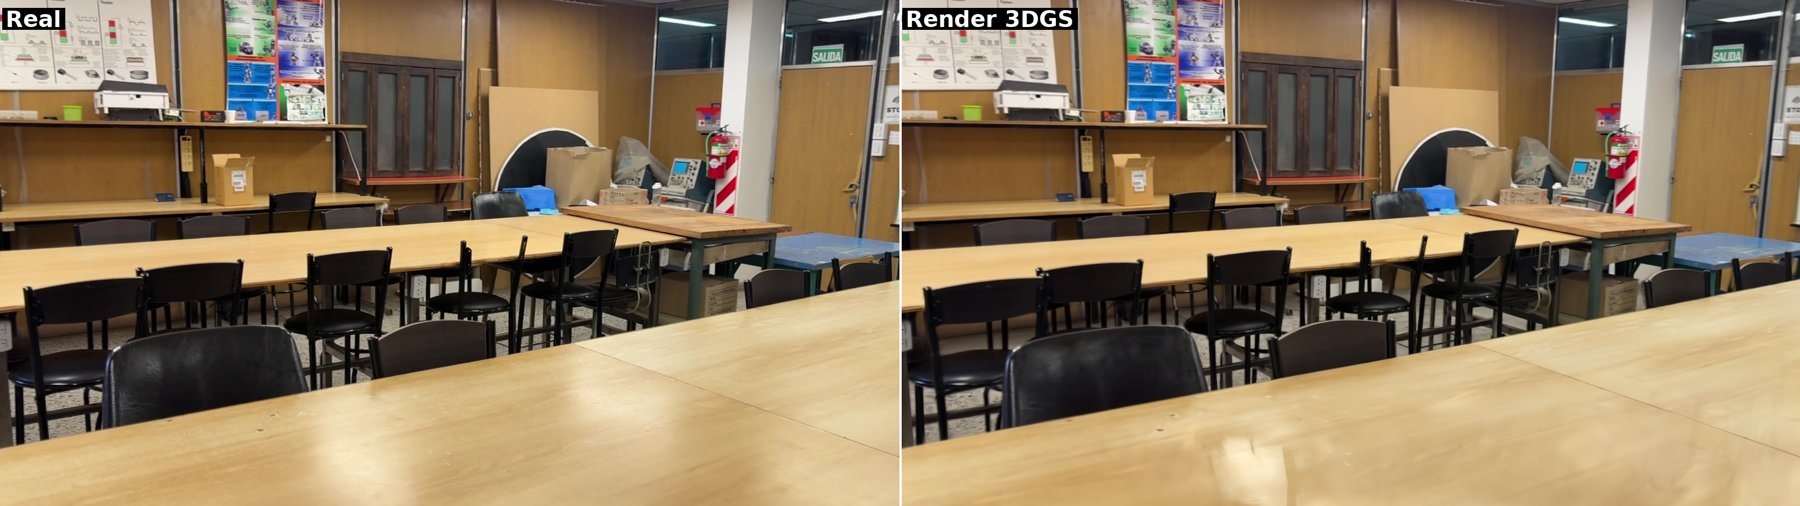
\includegraphics[width=0.49\textwidth]{fig/comp_aulab1.jpg}\hfill
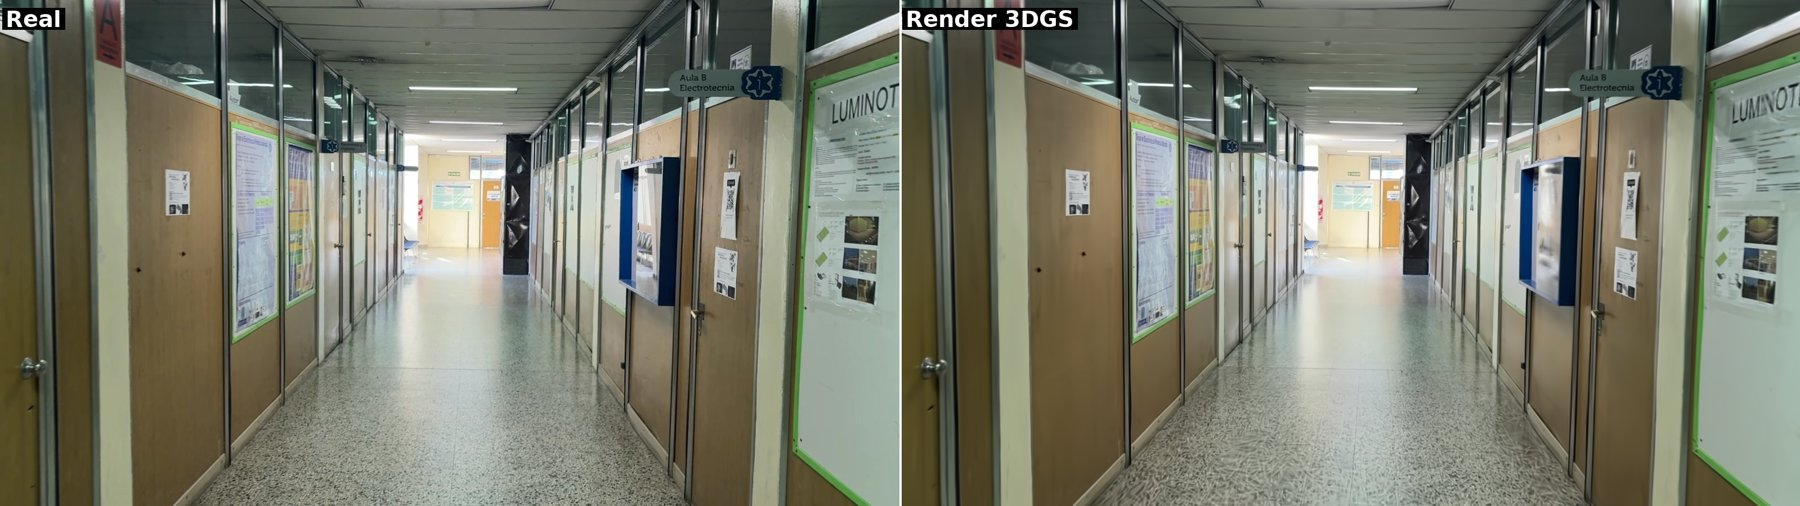
\includegraphics[width=0.49\textwidth]{fig/comp_pasillo.jpg}
\caption{Comparación entre la foto real (izquierda de cada par) y el render del modelo 3DGS (derecha), para un frame de evaluación no usado en el entrenamiento. Izquierda: Aula B1. Derecha: Pasillo.}
\label{fig:comp1}
\end{figure*}

\begin{figure*}[t]
\centering
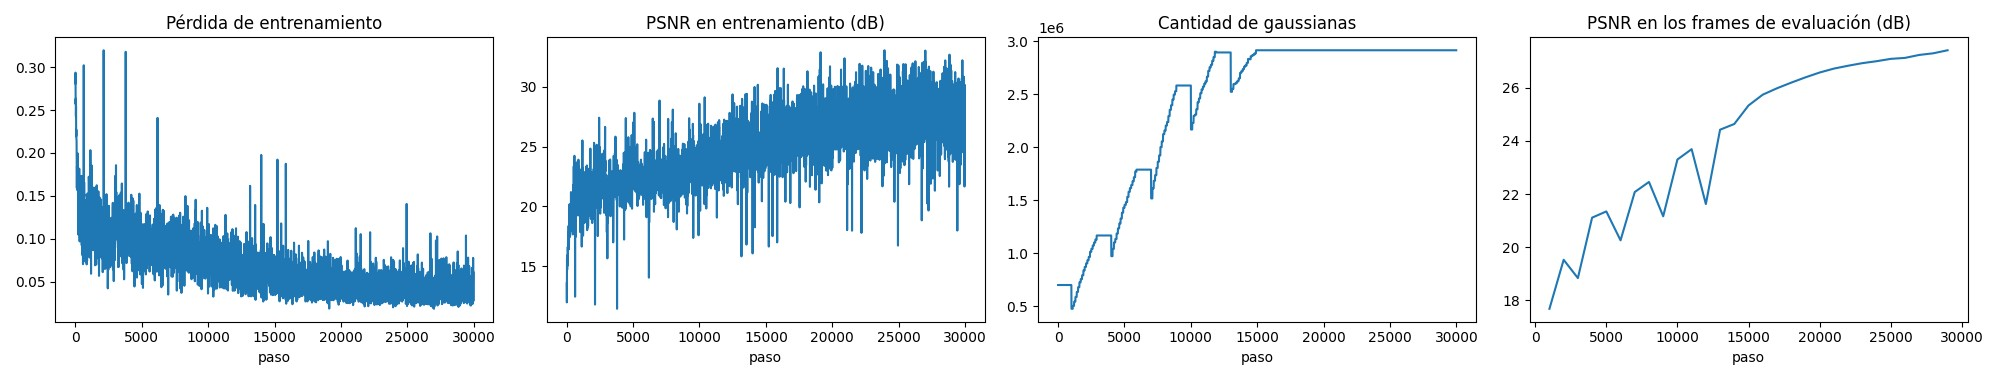
\includegraphics[width=0.95\textwidth]{fig/curvas_aulab2.jpg}
\caption{Curvas de entrenamiento en Aula B2: pérdida, PSNR de entrenamiento, cantidad de gaussianas y PSNR sobre los frames de evaluación.}
\label{fig:curvas}
\end{figure*}

\begin{figure}[htbp]
\centering
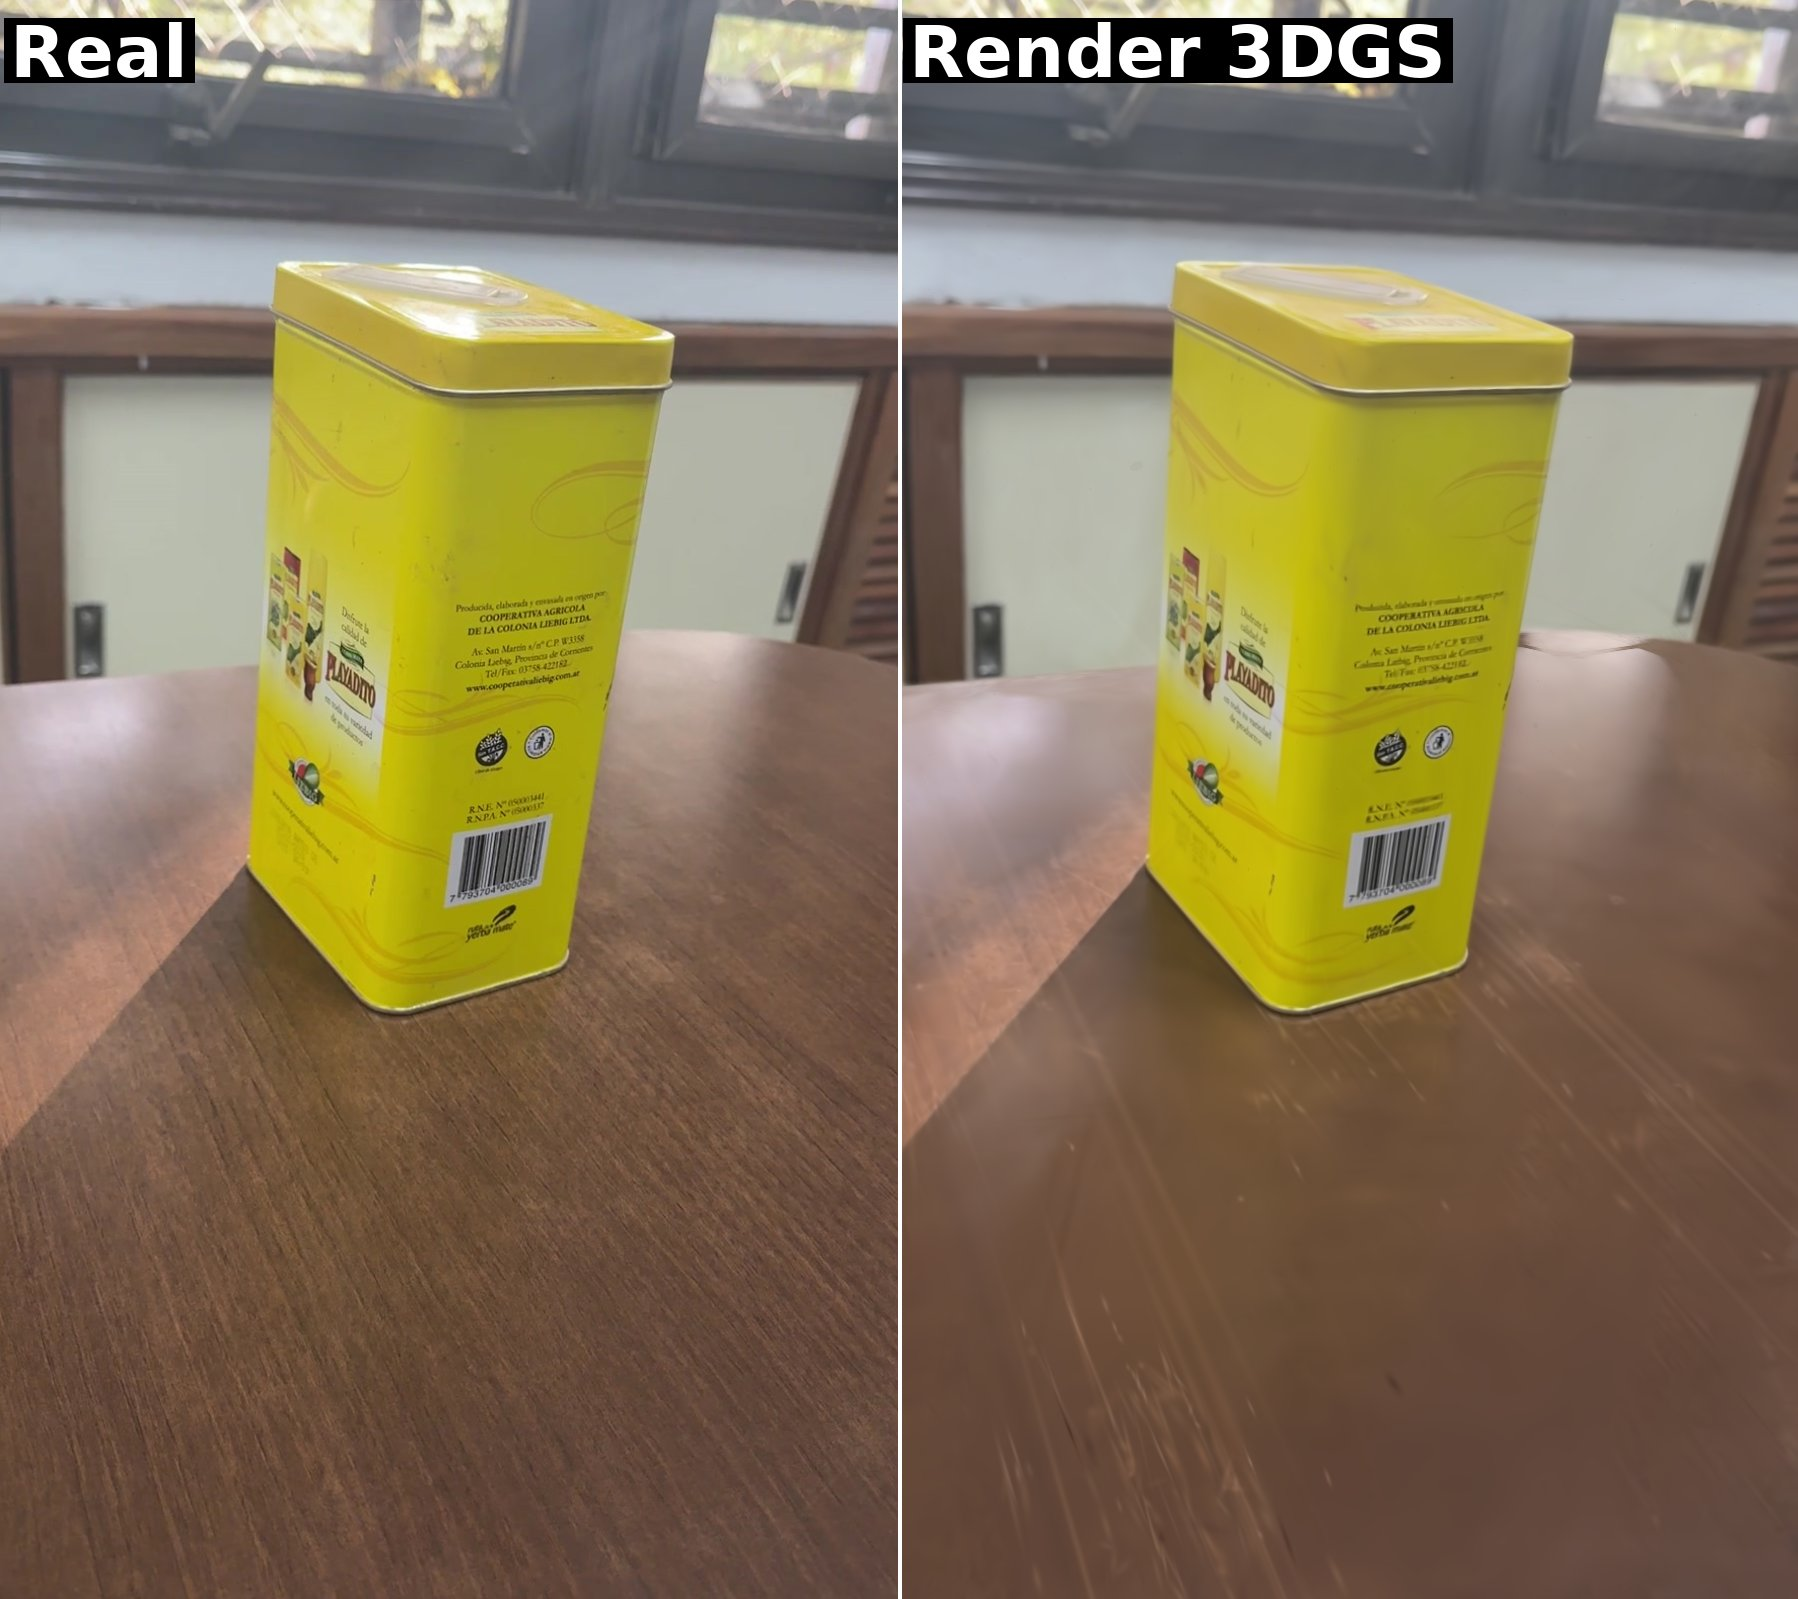
\includegraphics[width=0.49\columnwidth]{fig/comp_playadito.jpg}\hfill
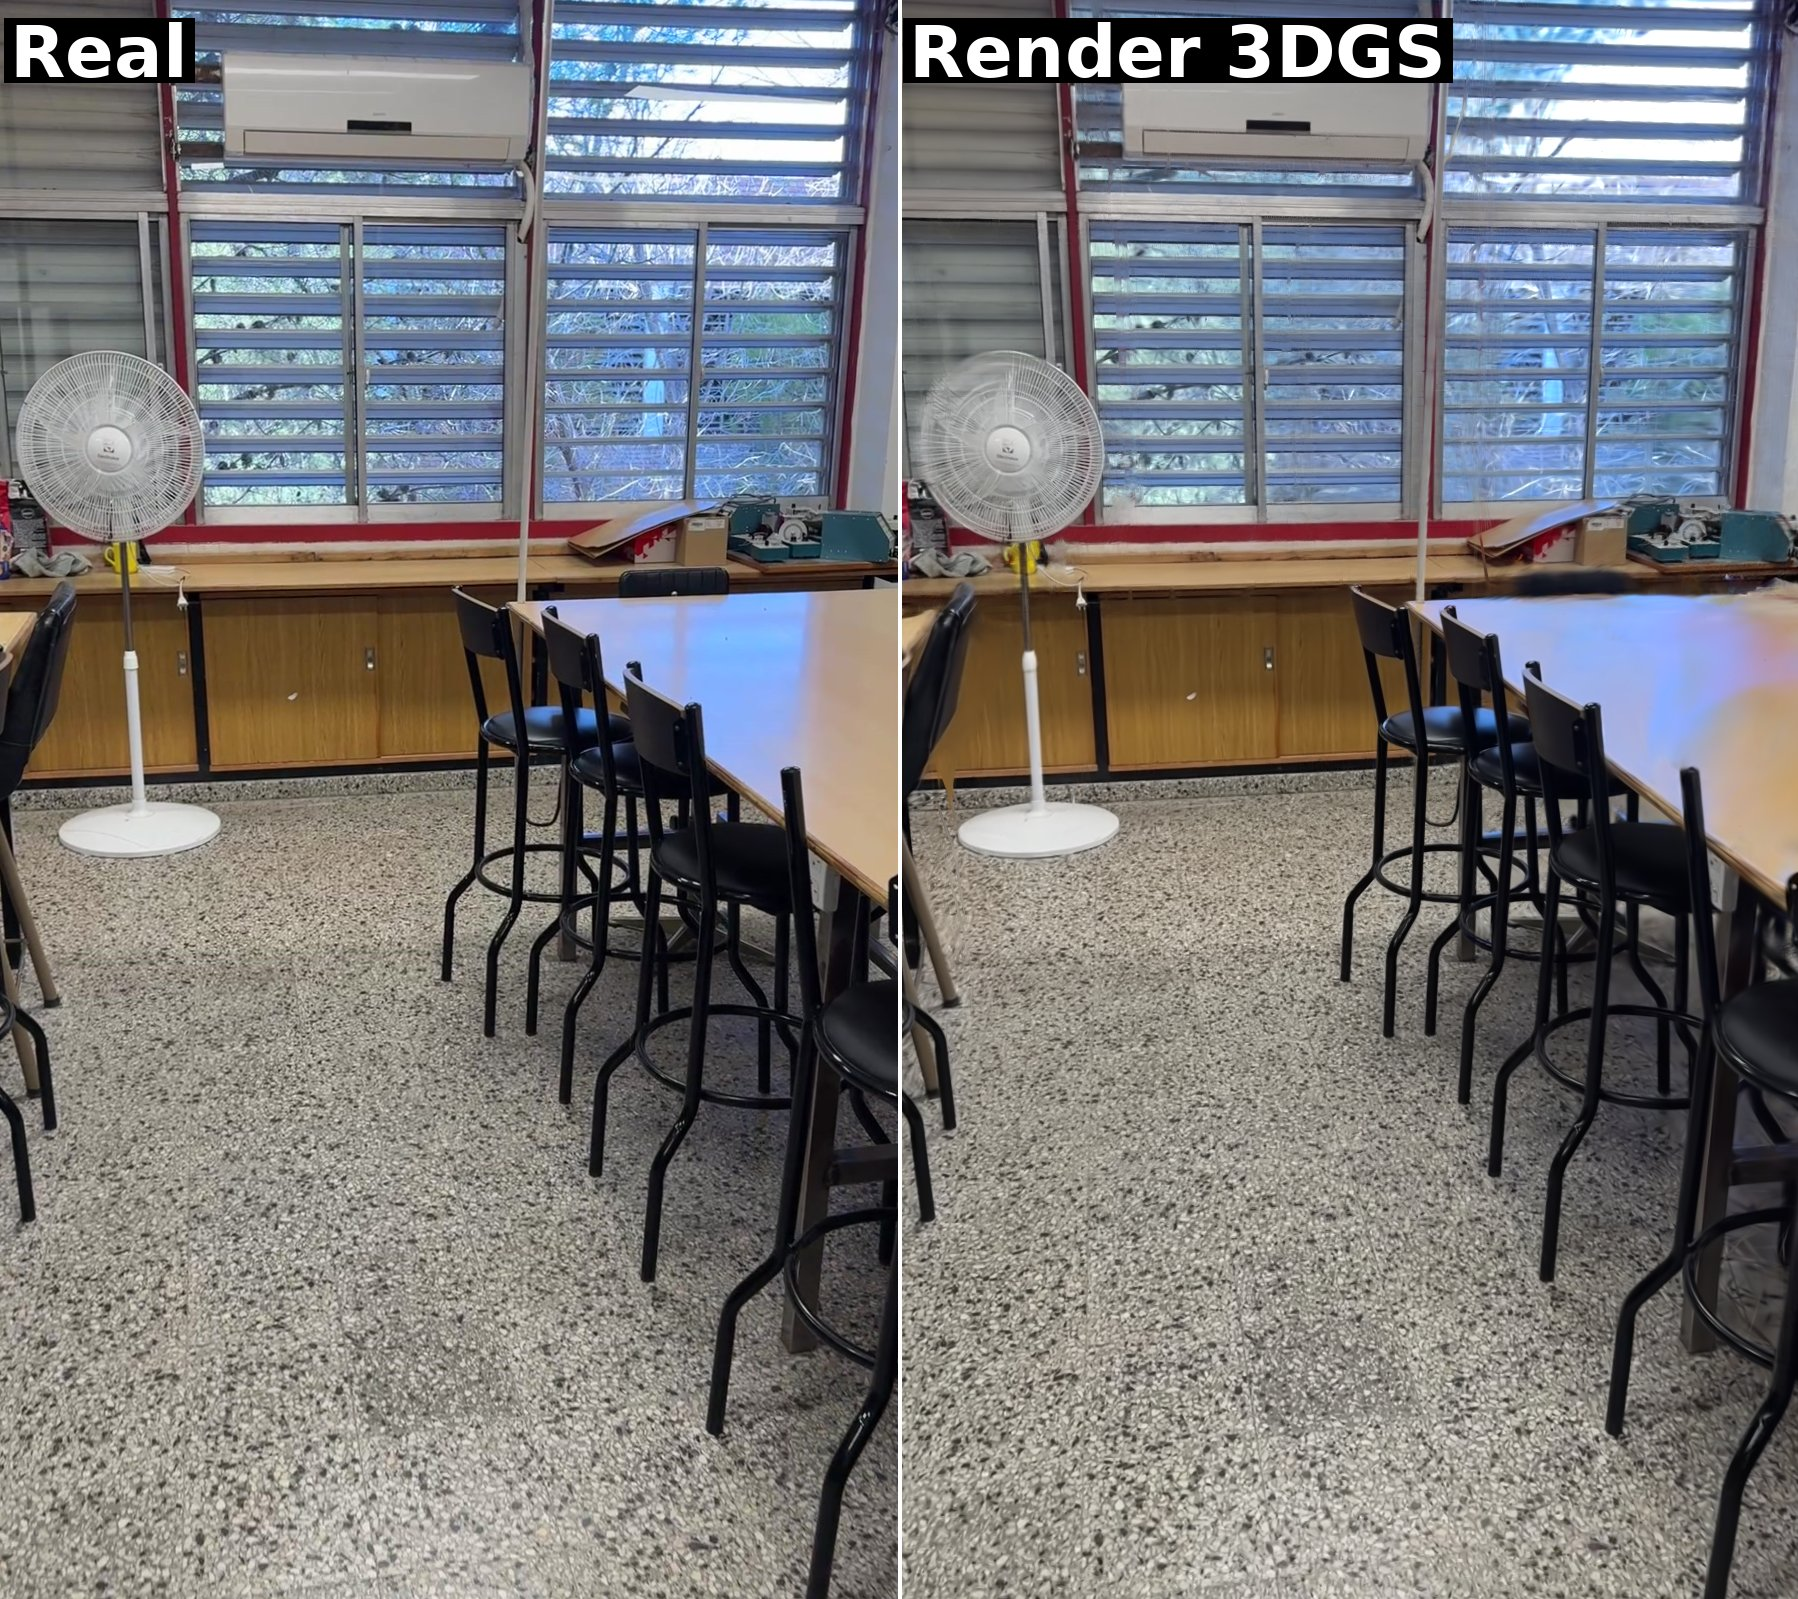
\includegraphics[width=0.49\columnwidth]{fig/comp_aulab2.jpg}
\caption{Foto real frente a render 3DGS en frames de evaluación. Izquierda: Lata. Derecha: Aula B2.}
\label{fig:comp2}
\end{figure}

Algunos resultados merecen comentarios:
\begin{itemize}
\item \textbf{Lata}: tiene el mayor PSNR pero el peor LPIPS. Gran parte de la imagen es la mesa de madera, de color casi uniforme, lo que favorece al PSNR. Sin embargo, el render pierde parte de la textura fina de la madera y no reproduce el reflejo del sol sobre la mesa, que cambiaba según el ángulo de la cámara. LPIPS es más sensible a esas diferencias de textura (Fig.~\ref{fig:comp2}).
\item \textbf{Aula B2}: es la escena más grande y la de peores métricas. El recorrido fue más largo (dos minutos de video), tuvo la mayor proporción de frames borrosos y las ventanas con luz exterior generan cambios de exposición entre frames. El modelo necesitó 2,86 millones de gaussianas (709\,MB).
\item \textbf{Aula B1 y Pasillo}: tienen los mejores LPIPS (alrededor de 0,10), con buena textura en paredes, carteles y muebles.
\end{itemize}

La Fig.~\ref{fig:curvas} muestra la evolución del entrenamiento en Aula B2. La pérdida disminuye y el PSNR de evaluación aumenta de forma sostenida. La cantidad de gaussianas crece durante la etapa de densificación y se estabiliza a partir de la iteración 15\,000, cuando esta se detiene. La Fig.~\ref{fig:gauss} muestra cómo quedaron las gaussianas del modelo final: vistas desde arriba dibujan la planta del aula, y la mayoría tiene opacidad cercana a 1 (son las que forman las superficies visibles) o cercana a 0 (aportan muy poco y son candidatas a podarse).

\begin{figure}[htbp]
\centering
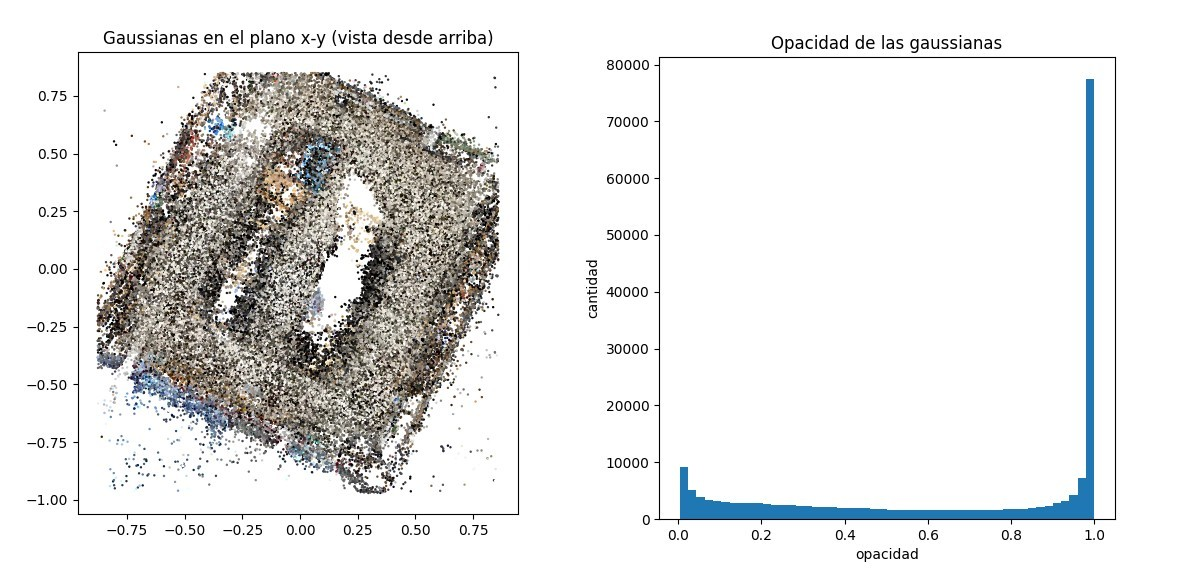
\includegraphics[width=\columnwidth]{fig/gauss_aulab2.jpg}
\caption{Gaussianas del modelo final de Aula B2. Izquierda: centros de una muestra de gaussianas vistos desde arriba, con su color; se reconoce la planta del aula y el recorrido central sin muebles. Derecha: histograma de la opacidad de las gaussianas.}
\label{fig:gauss}
\end{figure}


\section{Discusión}

El trabajo muestra que con un celular y procesamiento en la nube se puede obtener, entre media hora y tres horas según el tamaño de la escena, un modelo 3D de un entorno interior que se puede recorrer virtualmente. El pipeline aplica directamente los temas de la materia: el modelo de la cámara (Unidad II); la extracción de características con SIFT, las correspondencias y la eliminación de datos erróneos con RANSAC (Unidad III); y la estimación conjunta del movimiento de la cámara y de la estructura 3D, que es el problema de mapeo y localización simultánea resuelto en forma \textit{offline} (Unidad V).

\begin{figure}[htbp]
\centering
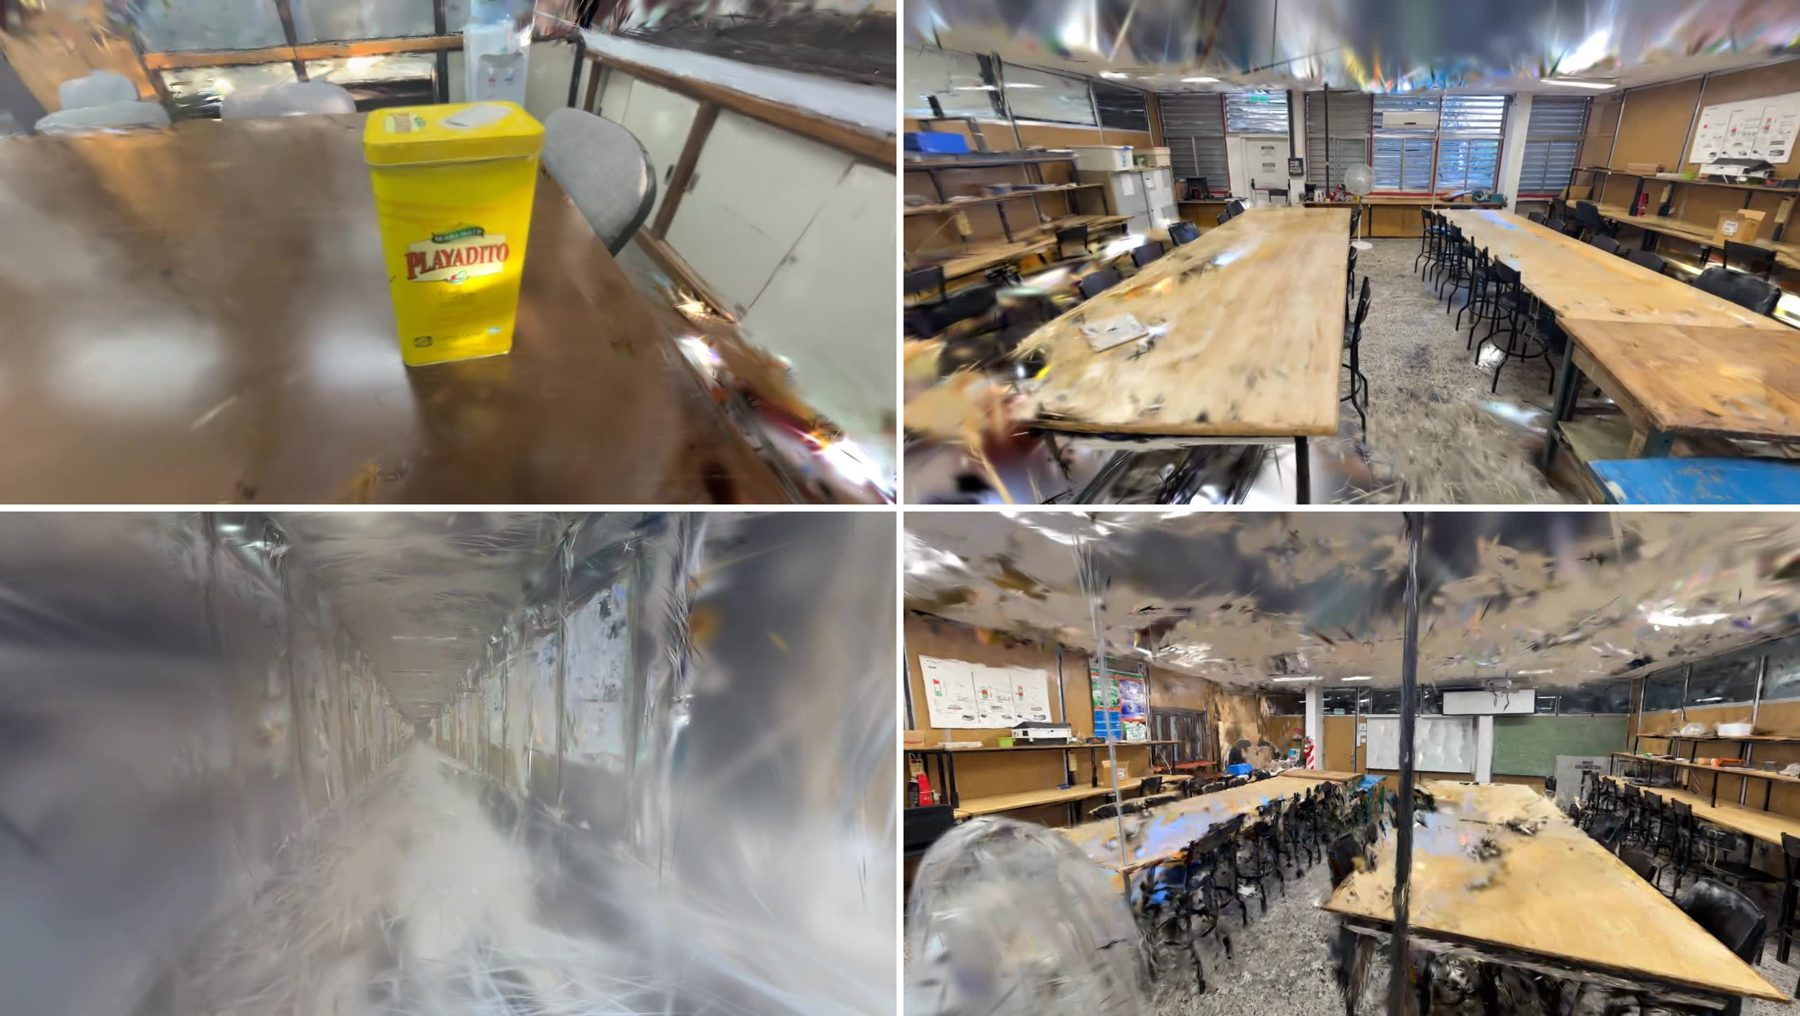
\includegraphics[width=0.88\columnwidth]{fig/vistas_nuevas.jpg}
\caption{Vistas renderizadas desde posiciones alejadas del recorrido de filmación (Lata, aulas y pasillo). Las zonas vistas desde pocos ángulos, como el techo y el piso cercano, muestran manchas y gaussianas flotantes.}
\label{fig:vistas}
\end{figure}

Las principales limitaciones encontradas son:
\begin{itemize}
\item \textbf{Métricas algo optimistas}: los frames de evaluación están intercalados con los de entrenamiento y son muy parecidos a ellos. Para puntos de vista alejados del recorrido filmado la calidad es menor y aparecen artefactos: manchas alargadas, techos y pisos ``borrosos'' y gaussianas flotantes (Fig.~\ref{fig:vistas}). Esto ocurre en zonas que la cámara vio desde pocos ángulos o que tienen poca textura.
\item \textbf{Escala}: al usar una cámara monocular el modelo no está en metros. Para usarlo en mediciones haría falta una referencia de longitud conocida o la \textit{fusión de datos} con otro sensor, por ejemplo la IMU del celular o un LiDAR.
\item \textbf{No es una malla}: las gaussianas son adecuadas para visualizar, pero no definen superficies sólidas. Para un simulador con colisiones (por ejemplo, Gazebo) haría falta convertir la escena en una malla.
\item \textbf{Escalabilidad del SfM}: en la escena más grande, la reconstrucción global tardó más de una hora y media. Usar menos frames o calcular correspondencias solo entre pares de imágenes más selectivos reduciría ese tiempo.
\item \textbf{Captura}: los frames borrosos, las superficies sin textura (paredes lisas, piso uniforme) y los cambios de iluminación (ventanas, reflejos) empeoran el resultado. Filmar despacio, con exposición fija y buena iluminación mejora la reconstrucción.
\end{itemize}

\section{Conclusiones}

Se reconstruyeron cuatro escenas reales a partir de video monocular combinando Structure from Motion y 3D Gaussian Splatting. El SfM registró el 100\,\% de los frames en todas las escenas, con errores de reproyección menores a 0,7 píxeles, y los modelos 3DGS alcanzaron entre 27,4 y 32,9\,dB de PSNR y SSIM entre 0,89 y 0,94 sobre frames no usados en el entrenamiento.

Usar la GPU para la extracción y la correspondencia de características redujo mucho esas etapas. En escenas grandes, el cuello de botella pasó a ser la reconstrucción global en CPU. Como trabajo futuro se propone recuperar la escala real del modelo, convertir la escena en una malla para usarla en simulación y evaluar el modelo con un recorrido de validación filmado aparte.

\begin{thebibliography}{9}

\bibitem{catedraU5}
Cátedra Introducción a los Vehículos Inteligentes, ``Unidad V: Aplicaciones (localización, construcción de mapas y SLAM),'' apuntes de clase, Facultad de Ingeniería, Universidad Nacional del Comahue, 2026.


\bibitem{catedraU2}
Cátedra Introducción a los Vehículos Inteligentes, ``Unidad II: Sensores típicos (LiDAR y cámara),'' apuntes de clase, Facultad de Ingeniería, Universidad Nacional del Comahue, 2026.


\bibitem{catedraU3}
Cátedra Introducción a los Vehículos Inteligentes, ``Unidad III: Extracción de características (RANSAC, puntos característicos, detectores, descriptores y correspondencias),'' apuntes de clase, Facultad de Ingeniería, Universidad Nacional del Comahue, 2026.


\bibitem{colmap}
J.~L. Schönberger, ``COLMAP: Structure-from-Motion and Multi-View Stereo,'' documentación oficial. [En línea]. Disponible: \url{https://colmap.github.io}


\bibitem{kerbl2023}
B.~Kerbl, G.~Kopanas, T.~Leimkühler y G.~Drettakis, ``3D Gaussian splatting for real-time radiance field rendering,'' \textit{ACM Transactions on Graphics}, vol.~42, no.~4, 2023. [En línea]. Disponible: \url{https://repo-sam.inria.fr/fungraph/3d-gaussian-splatting/}


\bibitem{nerfstudio}
Nerfstudio, ``Splatfacto,'' documentación oficial. [En línea]. Disponible: \url{https://docs.nerf.studio}

\end{thebibliography}

\end{document}
